\documentclass{article}

\usepackage[T1,T2A]{fontenc}
\usepackage[utf8]{inputenc}
\usepackage[english,russian]{babel}

\usepackage{pdfpages}
\usepackage{multirow}

\usepackage{caption}

\usepackage{amsmath}
\usepackage[hidelinks]{hyperref}


\usepackage{graphicx}%Вставка картинок
\graphicspath{{noiseimages/}}

\usepackage{float}%"Плавающие" картинки
\usepackage{wrapfig}%Обтекание фигур (таблиц, картинок и прочего)

\makeatletter
\def\@biblabel#1{#1. }
\makeatother

\setlength{\emergencystretch}{10pt}

\begin{document}

\begin{table}[ht]
\centering
\begin{tabular}{|c|c|}
\hline
			&Выход по току	\\
\hline
Поверхность при МГД стабильности &	\\
Момент времени $t_1$			&90.646	\\ 
Момент времени $t_2$		&93.594	\\  
\hline
Поверхность при выемке анодов &	\\
Момент времени $t_1$		&89.638	\\  
Момент времени $t_2$		&91.365	\\  
\hline
Поверхность при анодом эффекте &	\\
Момент времени $t_1$	&87.048	\\  
Момент времени $t_2$	&90.037	\\  
\hline
\end{tabular}
\caption{Выход по току $\eta$ для минимального значения МПР ($t_1 < t_2$). \label{table:vichPoToku}}
\end{table}


\begin{table}[ht]
\centering
\begin{tabular}{|c|c|}
\hline
			& Изменение потерь по току (\%)\\
\hline
МГД стабильный режим работы & 1.038	\\
\hline
Поверхность при выемке анодов &	1.799\\
\hline
Поверхность при анодом эффекте & 1.262	\\
\hline
\end{tabular}
\caption{Изменение потерь по току. \label{table:ismineniep}}
\end{table}

\begin{figure}[H]
\hspace*{-5cm}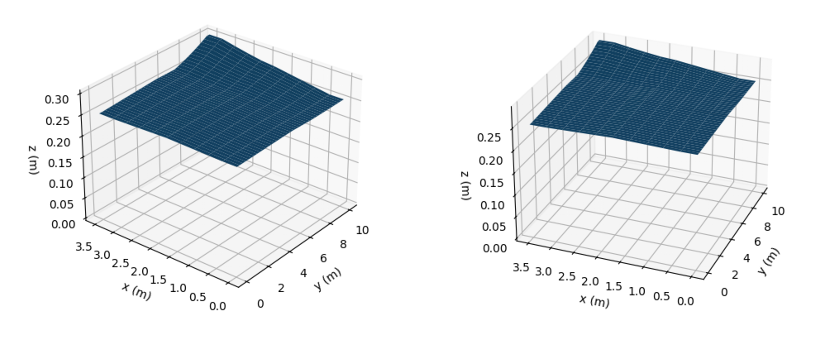
\includegraphics[scale=0.01]{спокойная.PNG}
\caption{МГД стабильный режим работы}
\end{figure}
\begin{figure}[H]
\hspace*{-5cm}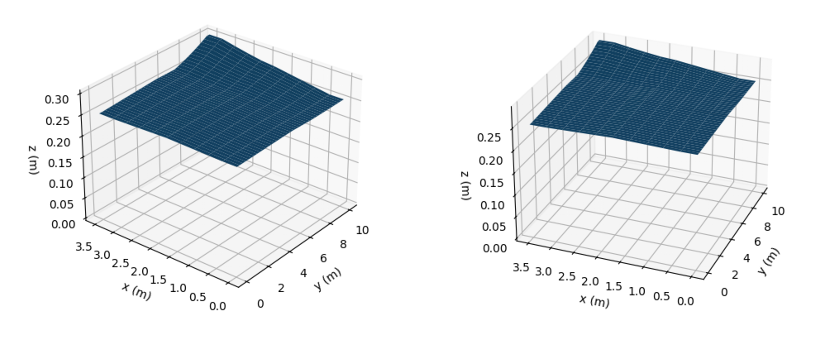
\includegraphics[scale=0.01]{спокойная.PNG}
\caption{МГД стабильный режим работы}
\end{figure}
\begin{figure}[H]
\hspace*{-5cm}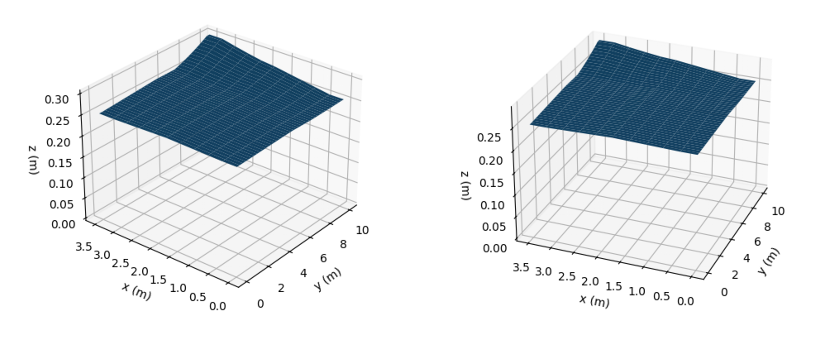
\includegraphics[scale=0.01]{спокойная.PNG}
\caption{МГД стабильный режим работы}
\end{figure}
\begin{figure}[H]
\hspace*{-5cm}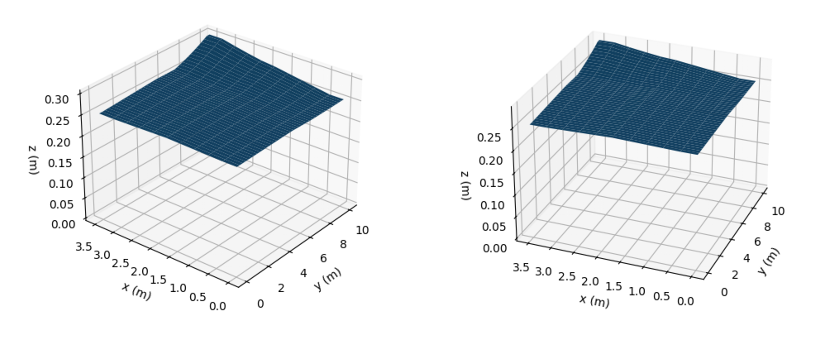
\includegraphics[scale=0.01]{спокойная.PNG}
\caption{МГД стабильный режим работы}
\end{figure}
\begin{figure}[H]
\hspace*{-5cm}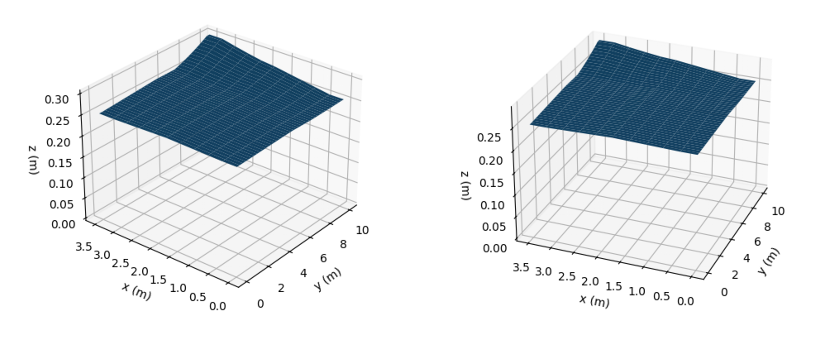
\includegraphics[scale=0.01]{спокойная.PNG}
\caption{МГД стабильный режим работы}
\end{figure}
\begin{figure}[H]
\hspace*{-5cm}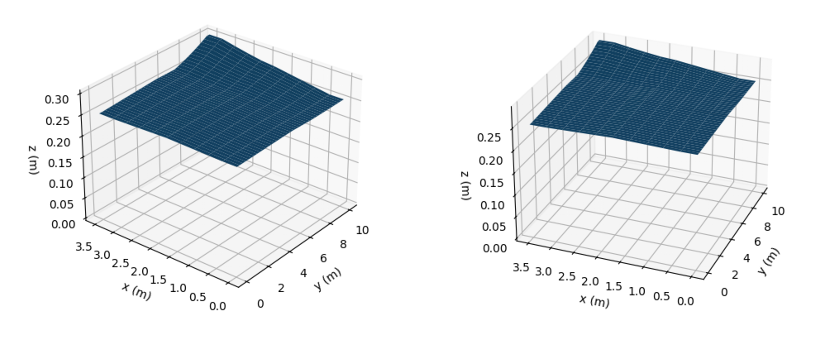
\includegraphics[scale=0.01]{спокойная.PNG}
\caption{МГД стабильный режим работы}
\end{figure}
\begin{figure}[H]
\hspace*{-5cm}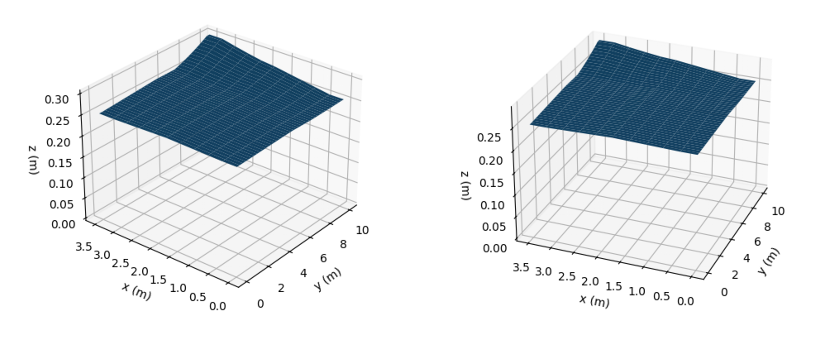
\includegraphics[scale=0.01]{спокойная.PNG}
\caption{МГД стабильный режим работы}
\end{figure}
\begin{figure}[H]
\hspace*{-5cm}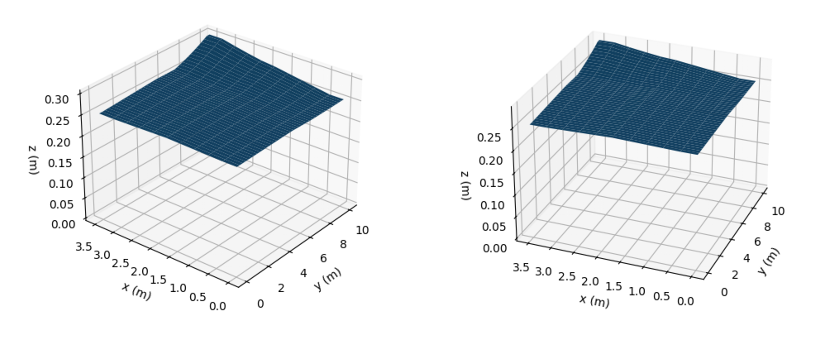
\includegraphics[scale=0.01]{спокойная.PNG}
\caption{МГД стабильный режим работы}
\end{figure}


\begin{figure}[H]
\hspace*{-5cm}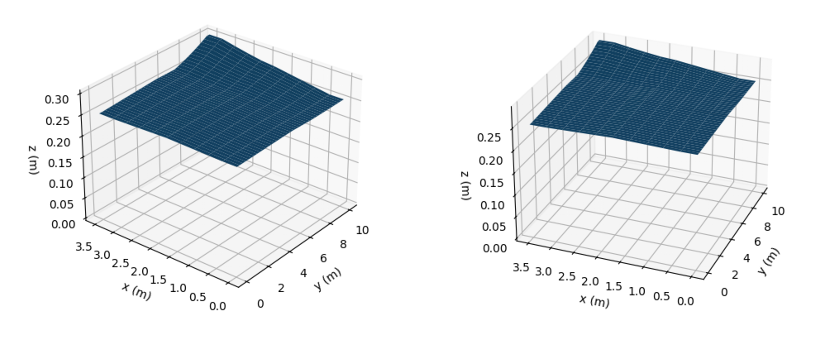
\includegraphics[width=200mm]{спокойная.PNG}
\caption{МГД стабильный режим работы}
\end{figure}

\begin{figure}[H]
\hspace*{-5cm}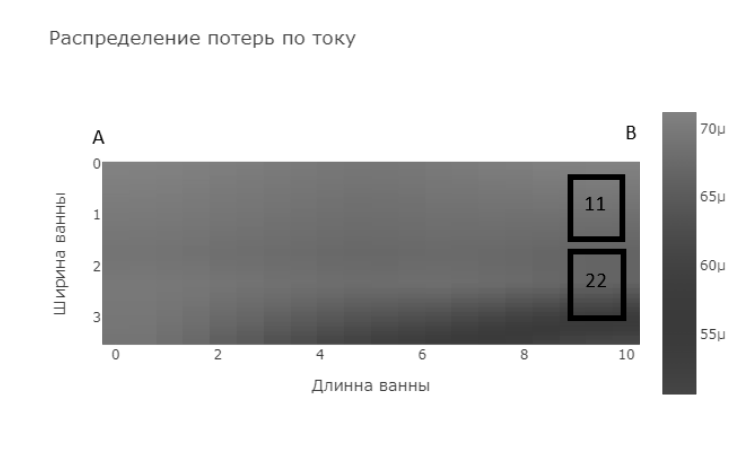
\includegraphics[width=180mm]{выемка анодов.PNG}
\caption{Поверхность при выемке анодов}
\end{figure}

\begin{figure}[H]
\hspace*{-5cm}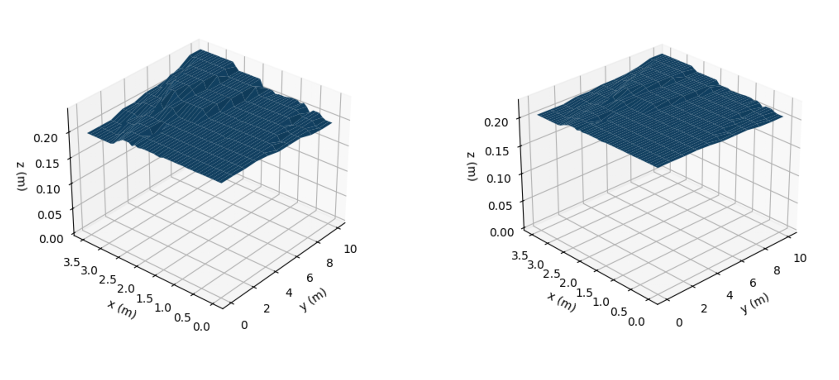
\includegraphics[width=180mm]{анодный эффект.PNG}
\caption{Поверхность при анодном эффекте}
\end{figure}

\end{document}